\section{Transformer}\raggedbottom \label{transformer}
Transformer sind eine spezifische Encoder-Decoder Deep Learning Architektur die insbesondere im Natural Language Processing eingesetzt wird. 
Basierend auf Attention Layern ermöglichen Transformer die Leistung bei vielen NLP Anwendungen stark zu steigern. 
Ein großer Vorteil von Transformermodellen ist die Parallelisierbarkeit. 
Hierdurch lassen sich extrem große Sprachmodelle, wie zum Beispiel BERT (\textbf{B}idirectional \textbf{E}ncoder \textbf{R}epresentations from \textbf{T}ransformers) oder GPT-2 (\textbf{G}enerative \textbf{P}re-trained \textbf{T}ransformer-2) auf Basis von Transformern trainieren. 
Beide Modelle erzielen auf den unterschiedlichsten Benchmarks hervorragende Ergebnisse.

Transformermodelle sind Sequence-To-Sequence Modelle, die aus einem Encoder und einem Decoder bestehen.
Die vortrainierten Sprachmodelle BERT und GPT-2 lassen sich auf spezielle Aufgabenbereiche Finetunen.


\subsection{Transformer Encoder / Decoder}
Transformer verwenden eine Encoder - Decoder Struktur. Der Encoder wandelt eine Eingabesequenz $(x_1,\ldots,x_n)$ in eine kontinuierliche Übergangsrepräsentation $(z_1, \ldots, z_n)$ um. 
Mit dieser Übergangsrepräsentation $z$ kann anschließlich vom Decoder eine Ausgabesequenz $(y_1, \ldots, y_n)$ generiert werden.
Der Transformer Decoder generiert Textsequenzen autoregressiv und bezieht also für die Berechnung des nächsten Ausgabetokens die vorherigen Tokens als Eingabe mit ein.


\begin{figure}[h]
    \label{transformerfig}
    \centering
    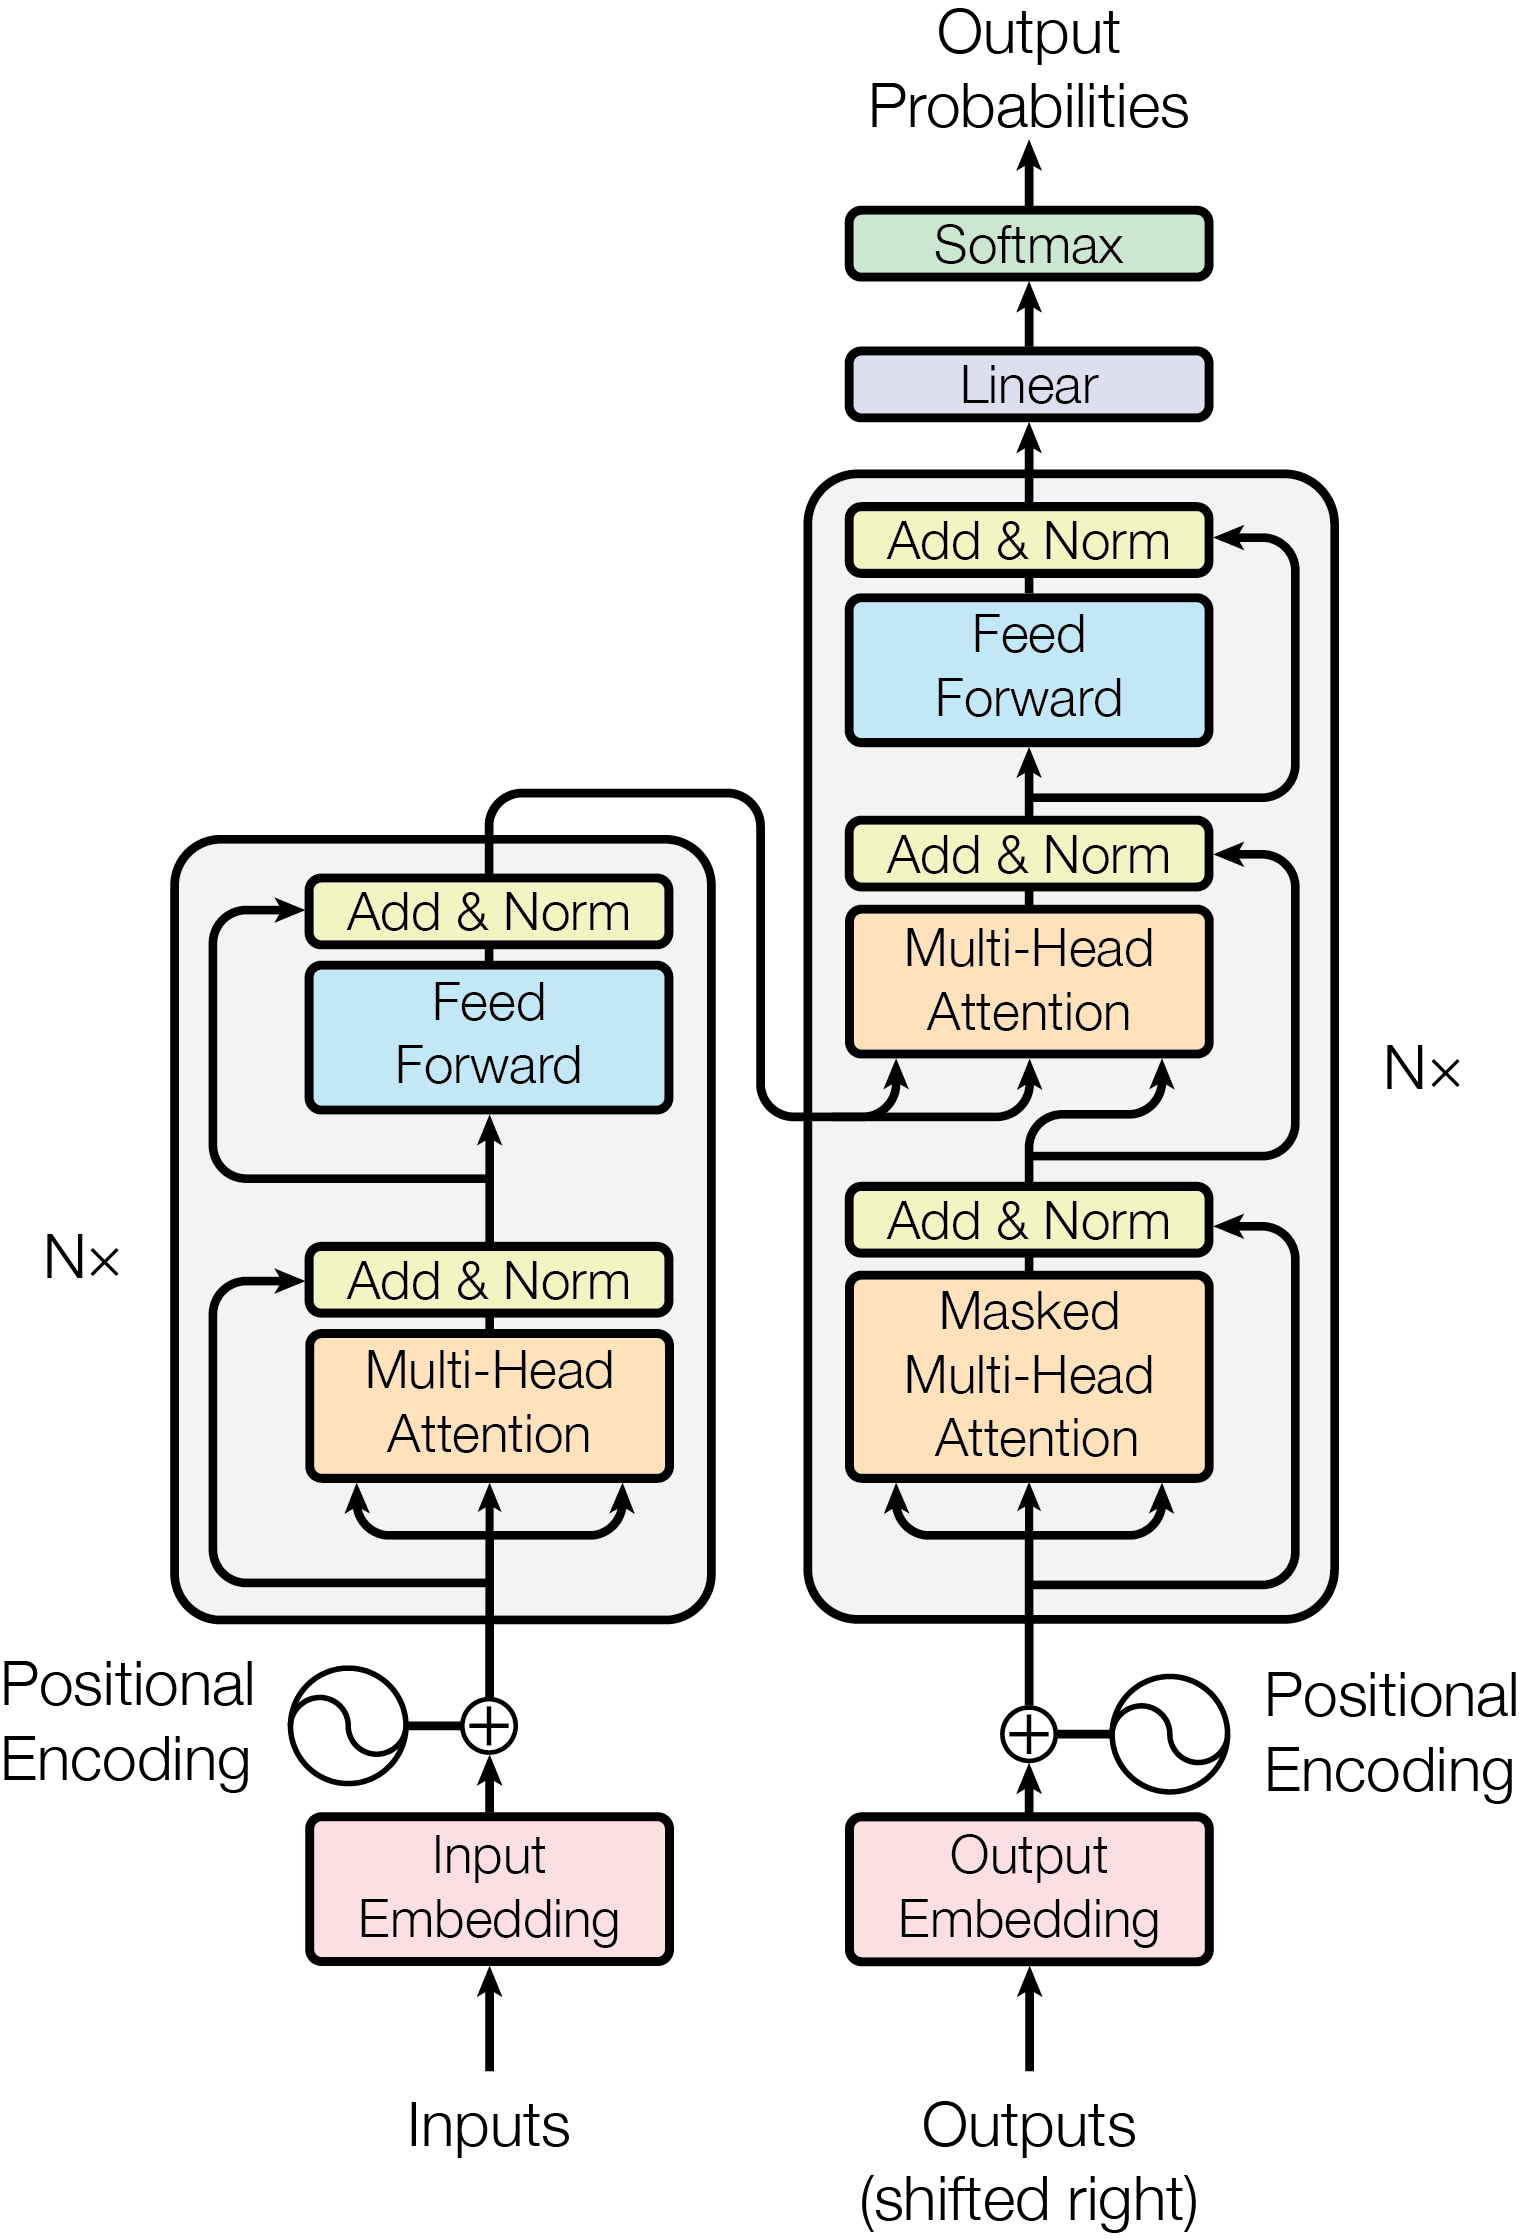
\includegraphics[width=8cm]{bilder/Transformer-Encoder-Decoder}
    \caption{Transformer Encoder (links) und Transformer Decoder (rechts)}
\end{figure}


Abbildung \ref{transformerfig} stellt die Architektur und den Datenfluss durch die verschiedenen Layer von Transformer Encodern und Decodern dar. 
Grundsätzlich bestehen sowohl der Encoder sowie auch der Decoder aus aufeinanderfolgenden Multi-Head Attention-Layern gefolgt von Fully-Connected Feed-Forward-Netzen.


Die Transformer Encoder Blöcke verwenden Self-Attention-Layer und beziehen damit ihre Eingabe vollständig aus der Ausgabe des vorherigen Layers. 
Die meisten Modelle verwenden mehrere Transformer Encoder Blöcke und Decoder Blöcke sequentiell hintereinander.

Nach Encodierung der Eingabesequenzen durch den Transformer Encoder wird die Ausgabe in Attention Key- und Value-Vektoren umgewandelt.
Diese Attentionvektoren werden vom Transformer Decoder in den Encoder-Decoder Attention Layern verwendet.
Im Gegensatz zu den Self-Attention-Layern der Encoder, verwendet der Decoder hier die Ausgabe des Encoders im Attention-Layer in den Berechnungen mit, um sich auf die korrekten Stellen im Input bei der Generierung der finalen Ausgabesequenz zu fokussieren.


%Stack
%encoder-decoder attention




\subsection{Attention-Layer} %Attnetnion nicht self attention
Durch die Attention-Layer von Transformermodellen lassen sich relevante Informationen erkennen und das Modell sich auf diese fokussieren. 
Der Attention-Layer innerhalb des Transformers berechnet die Relevanz von Values zu bestimmten Keys und Queries. 

Falls Attention-Layer ihre gesamte Eingabe wie bei Transformer Encodern aus einer Datenquelle beziehen sind diese Self-Attention-Layer.
Bei Self-Attention-Layern werden die Query- $(Q)$, Key- $(K)$ und Value- $(V)$ Vektoren aus dem Eingabevektor $(X)$ durch Multiplikation mit erlernten Gewichtsmatrizen $(W)$ generiert \citep{AttentionIALYN}. 
\begin{equation}
    Q = X \times W^{Q}, K = X \times W^{K}, V = X \times W^{V}
\end{equation}
Durch ein Dot-Product zwischen Query- und Key-Vektoren der entsprechenden Eingabewörtern mit anschließender Softmax Normalisierung lässt sich ein Score errechnen, der den Fokus im Valuevektor auf das jeweilige Wort angibt \citep{AttentionIALYN}.
\begin{equation}
    \label{attentioneq}
    Attention(Q,K,V) = Softmax(\frac{Q\times K^T}{\sqrt{d_k}})\times V
\end{equation}
In Gleichung \ref{attentioneq} werden die Berechnungen an den Matrizen $Q$ für die Queries, $K$ für die Keys und $V$ für die entsprechenden Values durchgeführt. Als Skalierungsfaktor wird $\sqrt{dk}$ , die Dimension der Key Vektoren verwendet, um einen stabilen Gradienten zu erhalten. 

Attention Funktionen lassen sich parallel ausführen. Diese Eigenschaft nutzen Transformermodelle aus und verwenden Multi-Head Attention Layer, um mehrere Attention Funktionen parallel ausführen.
Es werden parallel $h$ voneinander unabhängige Attention Layer ausgeführt, die Ihre einzelnen Ergebnisse für die Weiterverarbeitung aneinanderfügen und linear in die gewünschte Dimension transformieren. 
\begin{equation}
    \label{multiatteq}
    \begin{split}
    MultiHeadAttention(Q,K,V) &= [head_1, \ldots, head_h] \times W^{O} \\
    \text{mit } head_i &= Attention(QW_i^Q,KW_i^K,VW_i^V)
    \end{split}
\end{equation}
In Gleichung \ref{multiatteq} wird deutlich, dass die unterschiedlichen Attention-Heads voneinander unabhängig sind. Hierdurch können sich die einzelnen Attention-Heads auf unterschiedliche Merkmale in den Daten fokussieren.



    


\subsection{\textbf{B}idirectional \textbf{E}ncoder \textbf{R}epresentations from \textbf{T}ransformers}
BERT (\textbf{B}idirectional \textbf{E}ncoder \textbf{R}epresentations from \textbf{T}ransformers) ist ein von Google \citep{DBLP:journals/corr/abs-1810-04805} entwickeltes Encoder-Sprachmodell, welches sich durch die bidirektionale kontextuelle Einbettung von Worten auszeichnet.
Bei der Veröffentlichung von BERT konnten in vielen NLP Benchmarks Bestleistungen erzielt werden. 

BERT zeichnet sich ebenfalls durch die Möglichkeit des Transfer Learnings aus. Es existieren vortrainierte BERT-Sprachmodelle, die jeweils auf spezifische Aufgaben finegetuned werden können.

Die Modellarchitektur von BERT sind sequentielle Transformerencoderlayer. Das Basis BERT-Modell verwendet 12 Transformerencoderblöcke mit jeweils 12 Multi-Attention-Heads und einer Hidden-Size von 768.
BERT wird mit den beiden Pretrainings Aufgaben Masked Language Modeling und Next Sentence Prediction vortrainiert. Durch den besonderen Trainingsprozess betrachtet BERT Sequenzen von links und rechts gleichzeitig also bidirektional. Einige andere Verfahren betrachten Sequenzen nur einseitig, beziehungsweise kombinieren zwei einseitige Betrachtungen wie zum Beispiel ELMO \citep{elmo} und haben demnach keine tiefe bidirektionale Repräsentation der Sequenzen.

Beim Masked Language Modeling werden die bidirektionalen Repräsentationen trainiert indem zufällig 15\% der Worttokens in einer Sequenz gegen ein \textbf{[MASK]} Token ersetzt werden. Das Trainingsziel ist, die maskierten Tokens korrekt vorherzusagen.
Zum Verständnis der Zusammenhänge zwischen den Sätzen wird beim Next Sentence Prediction Pretrainingsschritt vorhergesagt, ob ein zu 50\% zufällig gewählter Satz B auf Satz A folgt \citep{DBLP:journals/corr/abs-1810-04805}.

\subsection{\textbf{G}enerative \textbf{P}re-trained \textbf{T}ransformer-2}
GPT-2 (\textbf{G}enerative \textbf{P}re-trained \textbf{T}ransformer-2) ist ein von OpenAI \citep{radford2019language} veröffentlichtes autoregressives Sprachmodell auf Basis von Transformerdecodern.
Autoregressive Sprachmodelle generieren Textsequenzen, indem sie einzeln Tokens generieren und diese an die Eingabesequenz anhängen. Die neue verlängerte Textsequenz wird erneut als Eingabe zur Generation genutzt.
Als generatives Modell erzielt es hervorragende Ergebnisse beim Generieren von kongruenten Textpassagen.

GPT-2 small besteht aus 12 sequentiellen Transformerdecodern.
Um die autoregressiven Eigenschaften beizubehalten, verwendet GPT-2 Masked Self-Attention Layer. 
Durch die Masked Self-Attention Layer kann das GPT-2 Modell beim Training im Gegensatz zu BERT lediglich die bereits bekannten Tokens betrachten.
%So lassen sich nacheinander jeweils einzelne nachfolgende Tokens zu einer Eingabesequenz generieren. 
%Im nächsten Schritt wird diese Eingabesequenz und das generierte Token als nächste Eingabe verwendet.

Zur Generation von Textpassagen kann GPT-2 unkontrolliert Samples aus einer leeren Eingabesequenz generieren.
Kontrolliert werden kann die Generation durch das Festlegen einer spezifischen Starteingabe an die GPT-2 generierte Tokens anfügt.

GPT-2 verwendet zur Tokenisierung das BytePairEncoding Verfahren \citep{bytepairencoding}.
Das Pretraining von GPT-2 wurde auf einem Datensatz mit ca. 8 Millionen Webseiten durchgeführt, mit der Aufgabenstellung jeweils in Texten das nächste Token vorherzusagen.



\pagebreak
